
%(BEGIN_QUESTION)
% Copyright 2006, Tony R. Kuphaldt, released under the Creative Commons Attribution License (v 1.0)
% This means you may do almost anything with this work of mine, so long as you give me proper credit

A basic circuit often used to regulate current through a variable-resistance load is the classic {\it current mirror}:

$$\includegraphics[width=15.5cm]{i00418x01.eps}$$

The ``programming'' resistor ($R_{prg}$) establishes the current magnitude to be maintained through the varying-resistance load, in this case an RTD or a thermistor.  For optimum performance, the two transistors should be precisely matched and also share the same heat sink (or be etched on the same semiconductor substrate).

However, we can do much better than this circuit if we use an operational amplifier.  Consider this ``modernized'' current mirror circuit:

$$\includegraphics[width=15.5cm]{i00418x02.eps}$$

Here there is no need for matched transistors or special heat-sinking.  So long as resistors $R_1$ and $R_2$ have equal resistance, the current through $R_{load}$ will be maintained at the same value as the current through $R_{prg}$.  If the intended current value is large, we may ``boost'' the output of the opamp with a single transistor:

$$\includegraphics[width=15.5cm]{i00418x03.eps}$$

Explain how both of these operational amplifier circuits work, and why they function as ``current mirrors.''

\underbar{file i00418}
%(END_QUESTION)





%(BEGIN_ANSWER)

I'll let you explain the working principle of both circuits!

%(END_ANSWER)





%(BEGIN_NOTES)


%INDEX% Measurement, temperature: current mirror circuit for RTDs and thermistors

%(END_NOTES)


